\documentclass[technicalreport]{ieicej}
\usepackage[dvipdfmx]{graphicx}
\usepackage[T1]{fontenc}
\usepackage{lmodern}
\usepackage{textcomp}
\usepackage{latexsym}
\usepackage{amsmath}
\usepackage{cite}
\usepackage{tikz}
\usepackage{geometry}
\usepackage{url}
\usepackage{schemabloc}
\usepackage{tikz}
\usepackage{makecell}
\usepackage{float}
\usetikzlibrary{arrows}

\usetikzlibrary{positioning,fit,calc}
\tikzset{block/.style={draw, thick, text width=1cm, minimum height=0.5cm, align=center}, line/.style={-latex}}  

\renewcommand{\figurename}{Fig.} % name the picture Fig.num
\renewcommand{\tablename}{Table } % name the table Table num
\renewcommand{\refname}{REFERENCE} % insert reference 

%调整文件显示位置和纸张
\geometry{
	a4paper,
	total={170mm,257mm},
	left=20mm,
	top=20mm,
}

\hoffset=-5mm
\voffset=-5mm

\def\IEICEJcls{\texttt{ieicej.cls}}
\def\IEICEJver{3.0}
\newcommand{\AmSLaTeX}{%
$\mathcal A$\lower.4ex\hbox{$\!\mathcal M\!$}$\mathcal S$-\LaTeX}
\def\BibTeX{{\rmfamily B\kern-.05em{\scshape i\kern-.025em b}\kern-.08em
T\kern-.1667em\lower.7ex\hbox{E}\kern-.125em X}}

\jtitle{M1課題レポート 第3回}
\jsubtitle{}
\etitle{Technical Report for M1 Labwork 3rd}
\esubtitle{}
\authorlist{
\authorentry[liuyuchen@radio.ict.e.titech.ac.jp]{劉 ゆしん}{Yuchen Liu}{Titech}
}

\affiliate[Titech]{東京工業大学 〒152-8550 東京都目黒区大岡山2-12-1}
{Tokyo Institute of Technology,~~2-12-1, O-okayama, Meguro-ku, Tokyo, 152-8550 Japan}

\begin{document}

\begin{eabstract}
In this third C workshop, we use C language to simulate fading in wireless communication due to delay and multi-path of transmission. In this workshop, we mainly simulate two fading channel: Rayleigh fading channel and frequency selective fading channel. First, we introduce the backgroud knowledege of these two fading channel. Next, we state the whole system desgin and simulation condition. Finally, we can see simulation BER performance of these two fading channel
\end{eabstract}

\maketitle

\section{Introduction}
Fading is attenuation of a signal in wireless communication caused by several factors. We can consider fading as a random process, which affects amplitude and phase of received signal. In this workshop, we mainly concentrate on two types of fading channel: Rayleigh fading channel and frequency selective fading channel. The full name of acronyms is summed in Table 1.\par
\subsection{Rayleigh Fading Channel}
Rayleigh fading is due to overlapping of multiple received radio waves at receiver. Power of received signal will stochastically fluctuates depending on distance to transmitter, time and mobility of receiver. The distribution of Rayleigh fading channel obeys joint of two independent and identically distributed Gaussian variables\cite{wireless_com}:
\begin{equation}
p(x,y)=\frac{1}{2\pi\sigma^2}{\rm exp}\left(-\frac{x^2+y^2}{2\sigma^2}\right)
\end{equation}
The amplitude of received signal obeys Rayleigh distribution:
\begin{equation}
p(r)=\frac{r}{\sigma^2}{\rm exp}\left(-\frac{r^2}{2\sigma^2}\right)
\end{equation}
And the phase of received signal obeys uniform distribution:
\begin{equation}
p(\theta)=\frac{1}{2\pi}
\end{equation}
The received signal $r(t)$ can be represented as follow:
\begin{equation}
r(t)=h(t,\tau)*s(t)+n(t)
\end{equation}
$h(t,\tau)$ in (4) is impulse channel response with $D$ paths, and $\tau$ is delay of each path. If $\tau$ is much smaller than one symbol time, it can be ingnored. Finally, the Rayleigh Fading Channel model can be written in the following form:
\begin{equation}
r(t)=\sum_{d=0}^{D-1}h_{d}(t)s(t)+n(t)
\end{equation}
When there is no delayed component, the Rayleigh channel can be regarded as a flat fading.
\begin{table}[H]
	\begin{center}
	\caption{ACRONYMS AND FULL MEANING}
	\begin{tabular}{|l|l|}
	\hline
	\textbf{Acronyms} & \textbf{Full Form} \\
	\hline
	 MLE & Maximum Likelihood Estimator  \\ 
	 \hline
	 QPSK & Quadrature Phase Shift Keying  \\ 
	 \hline
	 DQPSK & Differential Quadrature Phase Shift Keying  \\
	 \hline
	 BER & Bit Error Rate \\
	 \hline
	 SNR & Signal Noise Ratio \\ 
	 \hline
	 AWGN & Additive White Gaussian Noise \\ 
	 \hline
	 PDF & Probability Distribution Function \\
	 \hline
	 ISI & Inter Symbol Interference \\
	 \hline
	\end{tabular}
	\end{center}
\end{table}

\begin{figure}[H]
	\begin{center}
		\vspace{0cm}
		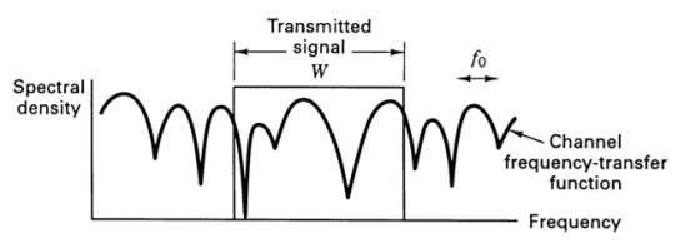
\includegraphics[width=\linewidth,clip]{fig/select_fading_illustrate.pdf}
		\caption{Impulse Response of Frequency Selective Fading Channel}
		\label{fig:sample}
	\end{center}
\end{figure}

\subsection{Frequency Selective Fading Channel}
Another important fading is frequency selective fading channel, which is also caused by overlapping of several delayed waves in different propagation paths. Compare to flat fading, the delay of each path in this fading exceeds one symbol time and will cause specific frequency attenuation in the bandwidth of transmission signal. The impulse response of frequency selective fading is shown in Fig. 1. If we suppose only two paths in channel, we can build channel model as follow:
\begin{equation}
r(i)=h_0s(i)+\underbrace{h_1s(i-1)}_{\rm ISI}+n(i)
\end{equation}
$h_0$ and $h_1$ are channel impulse response of each path.

\section{Simulation Desgin}
In this chapter we will introduce how to realize above two fading channel in C program and simulate BER performance with different Doppler shift.
\subsection{Design of Rayleigh Fading Channel Simulation}
Rayleigh fading channel can be represented in below form:
\begin{equation}
h(t)=\sum_{n=0}^{N-1}A_n{\rm exp}[j(2\pi f_D{\rm cos}\theta_nt+\phi_n)]
\end{equation}
$An$ is amplitude of impulse response which obeys 0 mean Gaussian distribution. $f_D=\frac{v}{\lambda}=\frac{vf_c}{c}$ is Doppler frequency which affects the rate of channel change over time. $\phi_n$ is initial phase which obeys uniform distribution. $N$ is number of waves, and if $N$ is large enough, according to Central Limit Theorem, $h(t)$ becomes 2 dimensional Gaussian distribution\cite{hoeffding1948central}. The theoretical BER of Rayleigh fading channel is\cite{ber}:
\begin{equation}
P_e(x)=\frac{1}{2}\left(1-\sqrt{\frac{x}{x+1}}\right)
\end{equation}
$x$ is SNR which is not in dB form.\par
To achieve best BER performance, receiver need to estimate channel state information to counteract amplitude attenuation and phase shift of receiving signal. However, even if we suppose the estimated channel is perfect, Rayleigh channel will change over time which is shown in Figure. 2. Thus, with Doppler shift, the BER of the receiving end cannot be close to the theoretical value according to (7).
\begin{figure}[tbp]
	\begin{center}
		\vspace{0cm}
		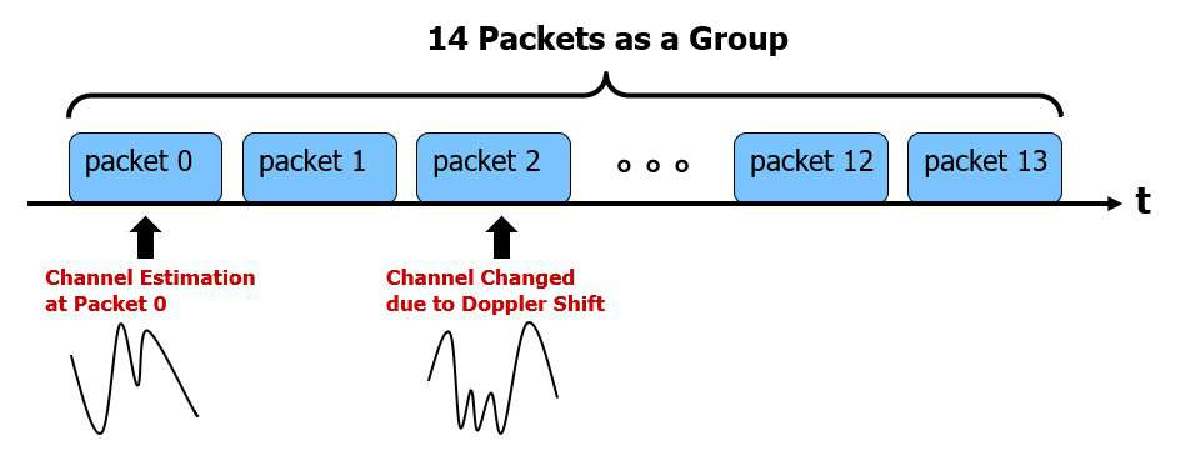
\includegraphics[width=\linewidth,clip]{fig/rayleigh_group.pdf}
		\caption{Illustration of Rayleigh Fading Channel}
		\label{fig:sample}
	\end{center}
\end{figure}

\begin{figure}[H]
	\begin{center}
		\vspace{0cm}
		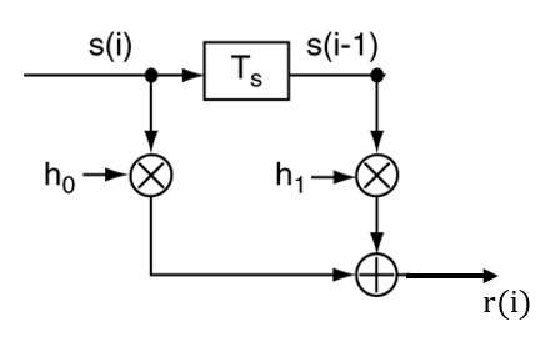
\includegraphics[width=\linewidth,clip]{fig/select_model.pdf}
		\caption{Illustration of Frequency Selective Fading Channel}
		\label{fig:sample}
	\end{center}
\end{figure}

\subsection{Design of Frequency Selective Fading Channel Simulation}
The generation process of frequency selective channel is illustrated in Fig. 3. Both $h_0$ and $h_1$ are generated as Rayleigh fading and each power is $\frac{1}{2}$ to let the power of the received signal be unit 1\cite{select}. 

\begin{table}[H]
	\begin{center}
	\caption{SIMULATION CONDITIONS}
	\label{tbl:simu}
	\small
	\begin{tabular}{ll}
	\hline
	ITEMS & CONDITIONS\\
	\hline
	Moduation Method & QPSK/DQPSK \\
	Transmission Bits & 128 \\
	Group Size & 14 \\
	Channel & Rayleigh Fading/Selective Fading Channel \\
	Detection & Noncoherent/Coherent Detection \\
	Number of Trials & $10^{4}$ \\
	Decision Method & MLE \\
	Channel Estimation & $\hat{h}=h$ \\
	Rayleigh Waves & 8 \\
	SNR Range & 0-30 dB \\
	\hline
	\end{tabular}
	\end{center}
\end{table}

\subsection{Simulation Result}
The simulation codition is listed in Table 2. BER performance of coherent demodulation in different Doppler shift in Rayleigh fading channel is shown in Fig. 4. We can see that QPSK and coherent demodualtion is not able to handle Rayleigh fading channel with Doppler shift, that the BER performance when $f_d$ is 1000 Hz is unacceptable. Then Fig. 5 shows theoretical and simulation BER curve of coherent demodulation and non-coherent demodulation without Doppler shift in Rayleigh fading channel, which we can see the simulation curve is quite consistent with the theoretical curve, and BER performance of coherent demodulation is 3 dB better than non-coherent demodulation. Fig. 6 shows BER performance of noncoherent demodulation in different Doppler shift. We can see that as the Doppler shift increases, the performance of BER gets worse.\par
Fig. 7 shows BER performance when Doppler shift is 0 Hz, 100 Hz and 1000 Hz in frequency selective channel. Due to ISI, system BER performance is worse than flat fading channel.

\begin{figure}[H]
	\begin{center}
		\vspace{0cm}
		\includegraphics[width=\linewidth,clip]{fig/r_coherent.eps}
		\caption{Coherent Demodulation BER with and without Phase Shift in Rayleigh Fading Channel}
		\label{fig:sample}
	\end{center}
\end{figure}

\begin{figure}[H]
	\begin{center}
		\vspace{0cm}
		\includegraphics[width=\linewidth,clip]{fig/without_fd.eps}
		\caption{Theoretic and Simulation BER without Doppler Shift in Rayleigh Fading Channel}
		\label{fig:sample}
	\end{center}
\end{figure}

\begin{figure}[H]
	\begin{center}
		\vspace{0cm}
		\includegraphics[width=\linewidth,clip]{fig/with_fd.eps}
		\caption{DQPSK and Noncoherent Demodulation BER with Different Doppler Shift in Rayleigh Fading Channel}
		\label{fig:sample}
	\end{center}
\end{figure}

\begin{figure}[H]
	\begin{center}
		\vspace{0cm}
		\includegraphics[width=\linewidth,clip]{fig/select.eps}
		\caption{DQPSK and Noncoherent Demodulation BER with Different Doppler Shift in Selective Fading Channel}
		\label{fig:sample}
	\end{center}
\end{figure}

\section{Conclusion}
In this workshop, we simulate BER performance in Rayleigh fading channel and frequency selective fading channel respectively. In summary of simualtion result, coherent demodulation performs better than noncoherent demodulation when there isn't any Doppler shift. However, BER performance of QPSK and coherent demodulation become unacceptable when Doppler shift appear. And in nonconherent demodulation, BER performance become worse as Doppler shift increases. In frequency selective fading channel, BER performance become much worse due to ISI. Thus, we need to deal with the special receiving method of this channel to achieve acceptable BER.

\bibliographystyle{IEEEtran}
\bibliography{rayleigh.bib}

\end{document} 